\documentclass[10pt,a4paper]{article}
\usepackage[T1]{fontenc}
\usepackage[utf8]{inputenc}
\usepackage{amsmath}
\usepackage{amsfonts}
\usepackage{amssymb}
\usepackage{listings}
\usepackage{graphicx}
\newcommand{\folge}[1]{\left \lbrace #1 \right \rbrace }
\lstset{language=Java, numbers=left, numberstyle=\footnotesize}
\author{Thorbjørn Christensen \\
Steffen Karlsson \\
Kai Ejler Rasmussen}
\title{Principles of Computer System Design - Assignment 2}
\begin{document}
\maketitle

\section*{Exercises}
\subsection*{Question 1: Serializability \& Locking}
\begin{figure}[ht]
\begin{minipage}[b]{0.50\linewidth}
\centering
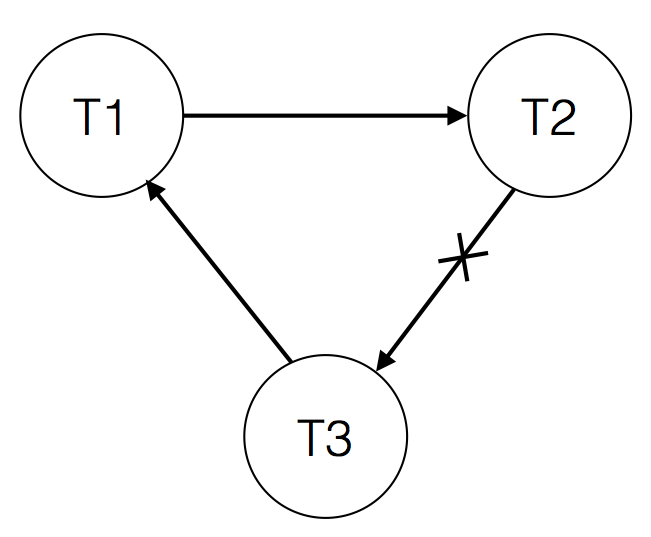
\includegraphics[width=\textwidth]{schedule1.png}
\end{minipage}
\hspace{0.5cm}
\begin{minipage}[b]{0.50\linewidth}
\centering
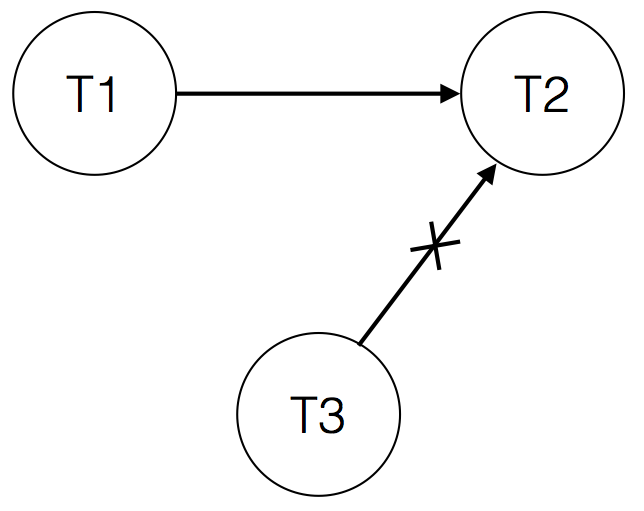
\includegraphics[width=\textwidth]{schedule2.png}
\end{minipage}
\caption{Precedence graph for the two schedules \label{fig:precedence-graph}}
\end{figure}

Figure \ref{fig:precedence-graph} depicts the precedence graphs for the two schedules. Both of these two schedules are conflict-serializable. 
\newline

In schedule two since T1 and T3 doesn't depend on each other at all, is there no chance of deadlock. Schedule one is a bit more tricky, the commit on T2 repeal the dependency between T1 and T2 and thereby the potential deadlock.

\begin{itemize}
\item Scenario 1: This scheduler could not be generated by a scheduler using strict 2PL, since T1 would not release the lock on $X$ before it commits, which means that T2 could not be scheduled to write to $X$ before the commit of T1.
 
\item Scenario 2: This schedule could have been generated by a scheduler using strict 2PL:

\begin{lstlisting}[numbers=none]
T1:     T2:     T3:
S(X)
R(X)            
                X(Z)
                W(Z)
                C
        S(Z)
        R(Z)
X(Y)
W(Y)
C
        X(X)
        W(X)
        X(Y)
        W(Y)
        C
\end{lstlisting}

where commit releases all the acquired locks.
\end{itemize}

\subsection*{Question 2: Optimistic Concurrency Control}
\subsubsection*{Scenario 1}
\texttt{T3} is not allowed to commit because of validation test 2, regarding $T_i$ completes before $T_j$ begins its write phase, which is validated by checking that the intersection between the write set of $T_i$ and the read set of $T_j$ is equal to the empty set (Ø). In other words is the intersection in this case between write set of \texttt{T2} and read set of \texttt{T3} not empty.
\newline

The conflicting element in the intersection is: 4.

\subsubsection*{Scenario 2}
\texttt{T3} is again not allowed to commit due to same reason as above, just between \texttt{T1} and \texttt{T3} instead of \texttt{T2}.
\newline

The conflicting element in the intersection is: 3.

\subsubsection*{Scenario 3}
\texttt{T3} is allowed to commit because of two times validation test 2, which where described in \textbf{Scenario 2}, \texttt{WS}(T1) $\cap$ \texttt{RS}(T3) = Ø and \texttt{WS}(T2) $\cap$ \texttt{RS}(T3) = Ø. Therefore does this scenario holds.

\subsection*{Questions for Discussion on the Concurrent Implementa- tion of Bookstore}

\begin{enumerate}
	\item Our locking protocol is based on strict 2 phase locking. Write or reads locks are acquired right before they are needed and all locks are released as the last call of the functions. A non-conservative 2PL is vulnerable to deadlocks which is explained below.
	\item We have implemented, as described, the strict 2PL locking protocol, which are vulnerable to deadlocks. We have tried to prevent it from happen, by sorting all inputs to the various methods, such that the acquisition of locks is in the same order each time. As an extension, what could have been implemented is the wait-for graph, which can abort cycles if they are detected (equal to a deadlock).
	\item A potential bottleneck in the system is that, when we insert a new book into the bookstore, we take a write lock on the whole \texttt{bookMap} and therefore it is only possible to insert one at a time. 
	\item The local implementation of using locks gives very little overhead compared to the possible concurrency. If only read request are requested, the number of concurrent request is equal to maximum number allowed threads which makes the overhead insignificant. However, write requests will block the concurrent read requests. Fortunately, read request are more likely to happen compared to write requests in this scenario.
\end{enumerate}

\section*{Test-cases}
All test cases for this assignment is placed in the file \texttt{ConcurrentBookStoreTest.java}:
\begin{itemize}
\item Test1: The \textbf{Test 1} as explained in the assignment text.
\item Test2: The \textbf{Test 2} as explained in the assignment text.
\item Test3:
Starting 10 threads each adding books to the bookstore concurrent. We tests that the number of the books when all threads are finished are as expected (that every thread manages to add all the books).
\item Test4:
We start 10 threads which each tries to add copies of different books in the bookstore (Thread 1 add copies to book 1 and thread 2 to book 2 ....) concurrent. We run through all books and tests that the number of copies are as expected on all 10 books. 
\end{itemize}
All the tests ran successfully, and every test fails when using an non-concurrent version of \texttt{ConcurrentCertainBookStore} (The initial version).

\end{document}